%we have some fixed parameters such as light control on or off. Mimics intersection lights.\\
%Whether simulated vehicles are able to turn or not.\\
%We have different max speeds - 60 or 40 km per hour approach. This translates to lower speeds %during turns (roughly half).\\

%tests are different combinations of above parameters. And results are measured in collisions, cars spawned, cars reaching destination, and time before deadlock.\\
%Deadlock is the situation where cars have been stuck for a period of time in the `intersection zone' without entering or leaving.

%To test the implementation of our system we ran some simulations 
To compare performances of the system over different paradigms and with different factors, we ran
multiple experimental simulations.
The factors that we changed over the different tests are from three classes: the paradigm, the speed of the cars, and the complexity.

For paradigm it is meant the use of  a traffic light regulated intersection versus a pure reactive approach.
When using traffic lights, the agents of the system still make use of their underlying reactive layer for obstacle avoidance, in the same way as they do without the traffic lights.
Traffic lights have the only purpose of regulating traffic flow by limiting its direction and changing it at fixed intervals.

Regarding complexity, it can be increased by allowing the cars to turn in order to reach any destination, or we can use a simpler system where cars only reach the opposite destination, going straigh.

The car speed is changed between three base cases: slow ( 30 km/h), medium (40 km/h) and fast (60 km/h).
For comparison, it is worth mentioning that the advised speed when making a 90 degree turn inside urban areas is around or below 30 km/h. %todo find reference

When simulating with traffic lights enabled, we test two intervals of time that regulate the duration of the green light.
We have an interval window of approximately 1 minute, that reflects a realistic scenario according to our observation of real life intersections.
We also test a much shorter window of 20 seconds, that should improve performance under the assumptions that:
\begin{enumerate}
\item autonomous vehicles can react faster than human drivers, so they can start moving immediately after the traffic light turns green compared to human drivers which could be slow or distracted;
\item shorter windows of time allow the traffic to be managed evenly, since traffic is evenly generated from the different directions.
\end{enumerate}

\subsection{Experimental results}

We measure performance of the systems mainly in terms of throughput, namely the amount of cars that get through the intersection per minute.
However, we also account for other factors, like the amount of collisions, the amount of deadlock situations, the time at which these occur and the frequency of these events.

A deadlock is the condition in which cars have been stuck in the intersection zone with no one entering or leaving for a period of time (about 10 seconds).

To test the implementation of our system we also account for information such as the number of cars spawned, number of cars "lost" (not reaching the correct destination) and the number of cars present in the intersection zone at the occurrence of a deadlock or collision.


On the other hand, we don't take into account neither fuel consumption nor gas emissions in this simulation, which would be relevant parameters for real life applications.

\subsubsection{Throughput}

\begin{figure}
\centering
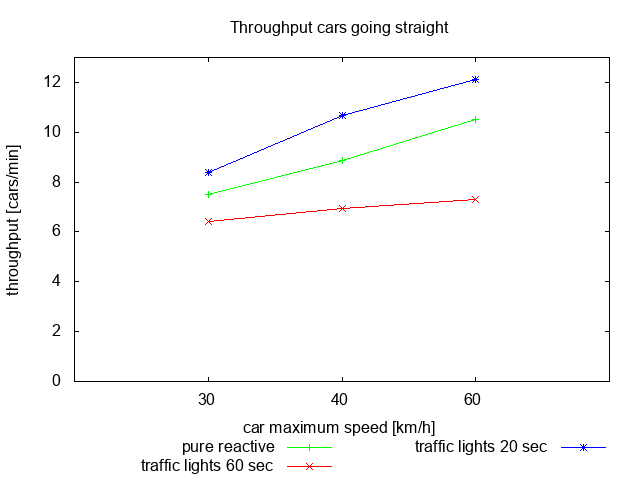
\includegraphics[scale=0.35]{img/plot_throughstraight}
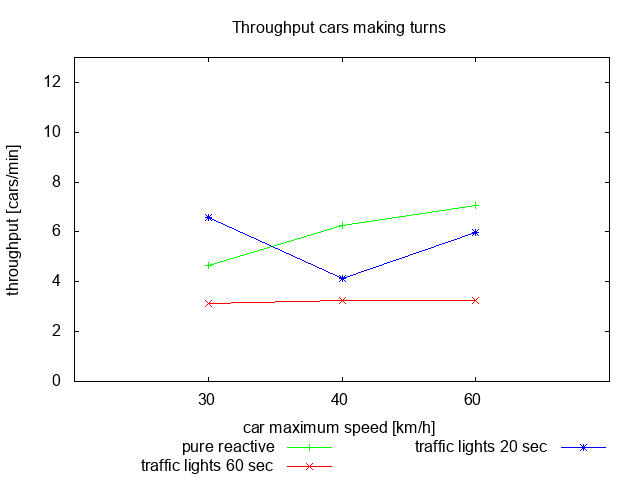
\includegraphics[scale=0.35]{img/plot_throughturns}
\caption{Throughputs in comparison: cars only move forward (left) versus cars able to turn (right). Pure reactive approach in green, traditional traffic light approach in red and fast traffic light approach in blue}
\label{fig:throughput}
\end{figure}

The graphs in figure \ref{fig:throughput} show the different throughputs of the system running with different factors.
%The graphs are divided by paradigm: the first one shows a pure reactive approach, while the second and the third one show the system working with traffic lights in intervals of 60 and 20 seconds respectively.
The graphs are divided by complexity: the first one shows the different throughputs when the cars can only go straight, while in the second one the cars can also make turns.

%For each graph, two versions of the same paradigm are compared: one where the agents only go straight and another one where they can turn in any directions.
For each graph, three paradigms are compared: the pure reactive approach, and the two with traffic lights, with light intervals of 60 and 20 seconds respectively.
Finally, for each case multiple tests are ran with cars moving at different speeds, that are represented on the x axis.
\newline

The first thing that can be evinced from the graphs is that when adding complexity, namely the ability to turn, throughput drops in all three cases.
%This can be easily seen in the fact that in every graph the darkest line (cars going straight) is above the lightest one.


This is mostly due to the fact that deadlocks are produced at a higher rate when turning is enabled, as will be later discussed.

The main purpose of the graph though, is the comparison between the pure reactive approach (green), the traffic light approach (red), and the approach with traffic lights with a faster switch interval (blue).

In the first graph the pure reactive approach achieves better throughput than the traditional traffic light approach, but they are both surpassed by the faster traffic light system.

When the cars can turn, throughput is lowered by approximately half, and the pure reactive seems to be the best system, followed by the fast traffic-light system and the traditional one in last position.

\subsubsection{Deadlocks}

\begin{figure}
\centering
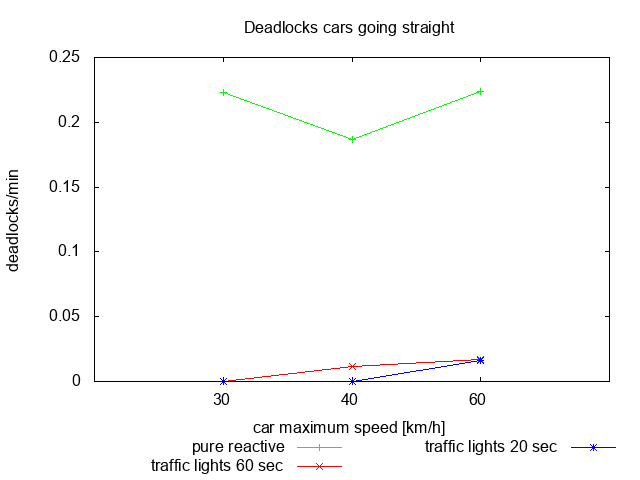
\includegraphics[scale=0.35]{img/plot_deadlocksstraight}
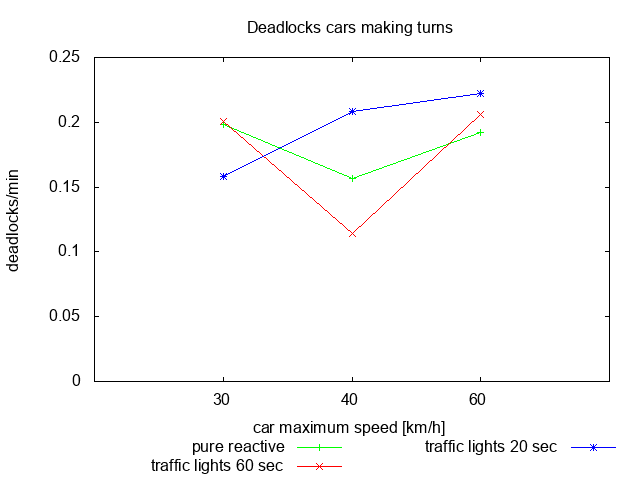
\includegraphics[scale=0.35]{img/plot_deadlocksturns}
\caption{Deadlocks' frequencies in comparison}
\label{fig:deadlocks}
\end{figure}

\begin{figure}
\centering
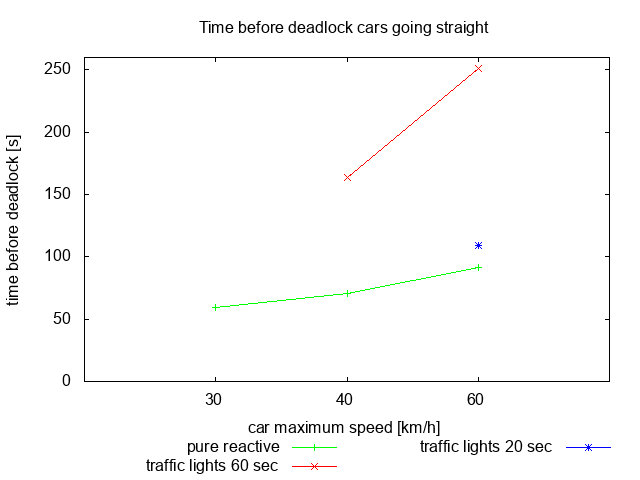
\includegraphics[scale=0.35]{img/plot_dtimestraight}
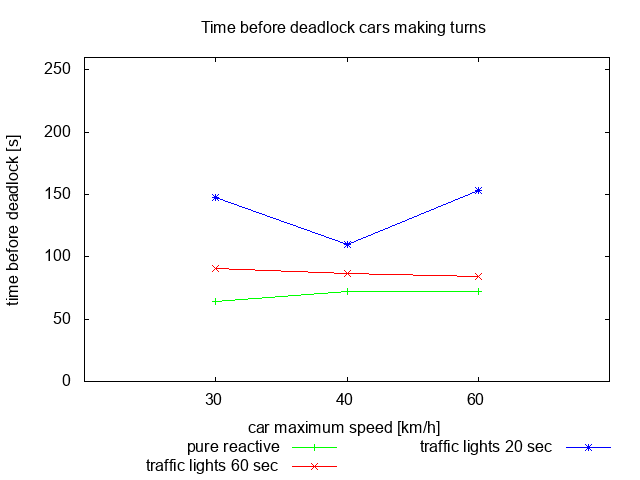
\includegraphics[scale=0.35]{img/plot_dtimeturns}
\caption{Time before deadlock in comparison}
\label{fig:dtime}
\end{figure}

Figure \ref{fig:deadlocks} shows the occurrence of deadlocks per minute in the various simulations.\\
Figure \ref{fig:dtime} shows the average time before a deadlock occurs.
It is clear from these graphs that when the cars can only go forward, deadlocks are much more frequent in the pure reactive system.
Not only they happen more, but are likely to occur in less time.

When cars can turn, deadlocks are frequent for every study case, at a comparable level.
The only case when values differ significantly is when cars move at an average speed, while when they move slow or fast they present similar behaviours.
In regards to the times, deadlocks are likely to happen in less time for the pure reactive approach, while the system that can last the longest is the fast traffic-light one.


\subsubsection{Discussion}
These results 


\subsubsection{Collisions}


\begin{figure}
\centering
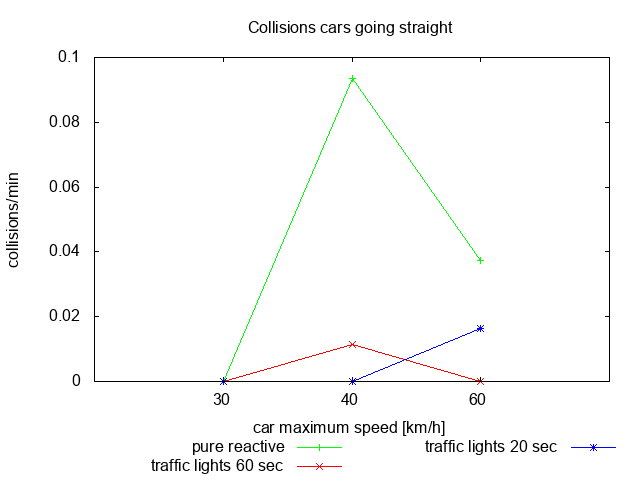
\includegraphics[scale=0.35]{img/plot_collisionsstraight}
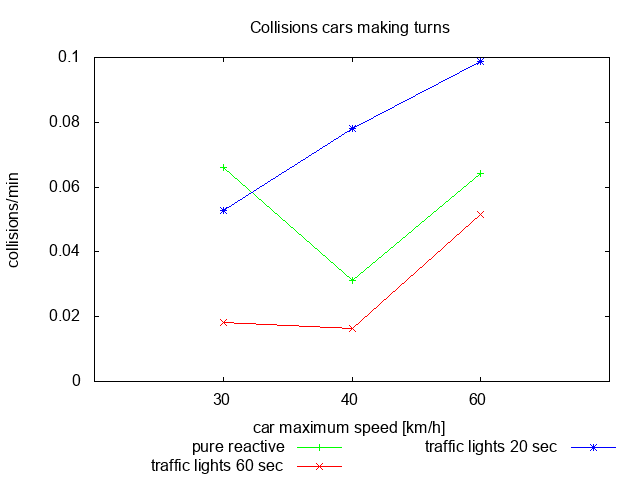
\includegraphics[scale=0.35]{img/plot_collisionsturns}
\caption{Collisions in comparison}
\label{fig:collisions}
\end{figure}




